\documentclass[14pt]{extbook}
\usepackage{multicol, enumerate, enumitem, hyperref, color, soul, setspace, parskip, fancyhdr} %General Packages
\usepackage{amssymb, amsthm, amsmath, latexsym, units, mathtools} %Math Packages
\everymath{\displaystyle} %All math in Display Style
% Packages with additional options
\usepackage[headsep=0.5cm,headheight=12pt, left=1 in,right= 1 in,top= 1 in,bottom= 1 in]{geometry}
\usepackage[usenames,dvipsnames]{xcolor}
\usepackage{dashrule}  % Package to use the command below to create lines between items
\newcommand{\litem}[1]{\item#1\hspace*{-1cm}\rule{\textwidth}{0.4pt}}
\pagestyle{fancy}
\lhead{Progress Quiz 6}
\chead{}
\rhead{Version C}
\lfoot{9689-6866}
\cfoot{}
\rfoot{Spring 2021}
\begin{document}

\begin{enumerate}
\litem{
Graph the equation below.\[ f(x) = -(x+3)^2 - 15 \]\begin{enumerate}[label=\Alph*.]
\begin{multicols}{2}\item 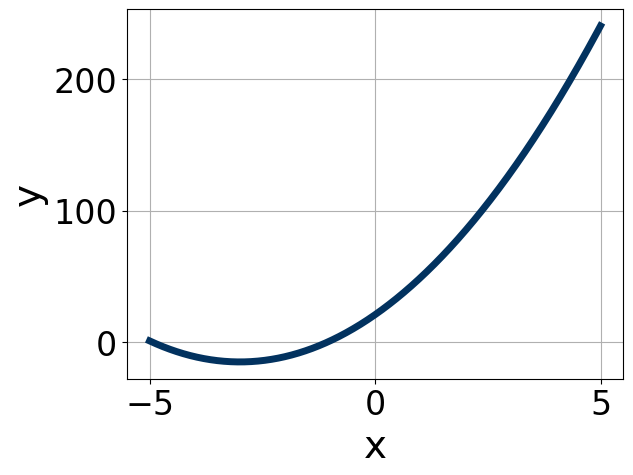
\includegraphics[width = 0.3\textwidth]{../Figures/quadraticEquationToGraphAC.png}\item 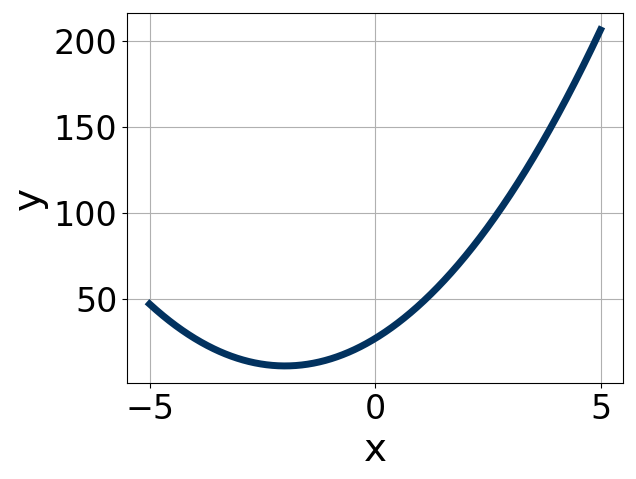
\includegraphics[width = 0.3\textwidth]{../Figures/quadraticEquationToGraphBC.png}\item 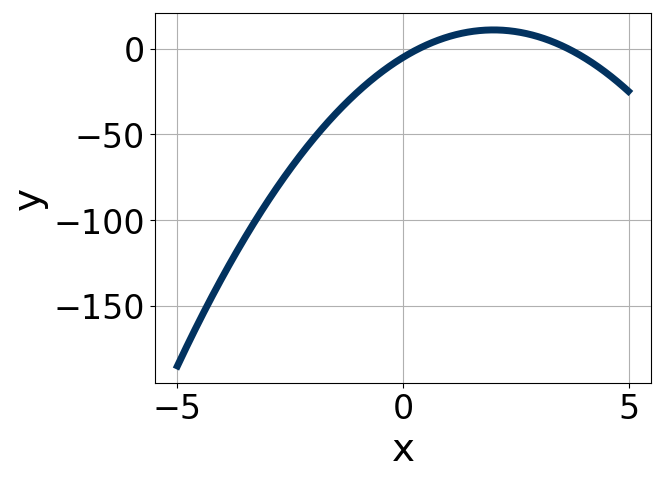
\includegraphics[width = 0.3\textwidth]{../Figures/quadraticEquationToGraphCC.png}\item 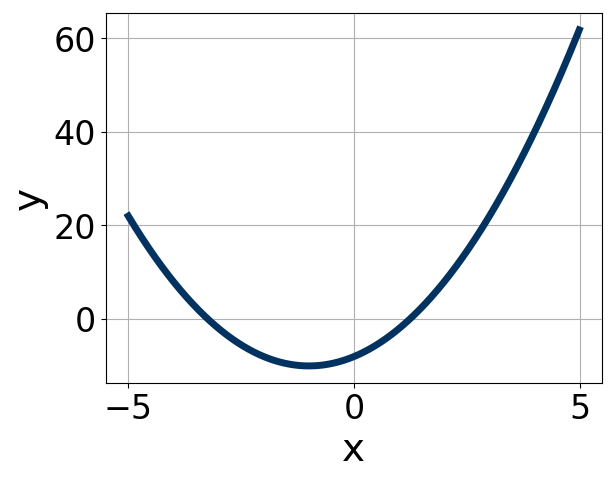
\includegraphics[width = 0.3\textwidth]{../Figures/quadraticEquationToGraphDC.png}\end{multicols}\item None of the above.
\end{enumerate} }
\litem{
Solve the quadratic equation below. Then, choose the intervals that the solutions belong to, with $x_1 \leq x_2$ (if they exist).\[ 13x^{2} -15 x -9 = 0 \]\begin{enumerate}[label=\Alph*.]
\item \( x_1 \in [-25.8, -25.1] \text{ and } x_2 \in [26.9, 27.9] \)
\item \( x_1 \in [-0.8, -0.2] \text{ and } x_2 \in [0.59, 5.59] \)
\item \( x_1 \in [-2, -1] \text{ and } x_2 \in [-1.56, 1.44] \)
\item \( x_1 \in [-6.2, -4] \text{ and } x_2 \in [20.66, 21.66] \)
\item \( \text{There are no Real solutions.} \)

\end{enumerate} }
\litem{
Solve the quadratic equation below. Then, choose the intervals that the solutions $x_1$ and $x_2$ belong to, with $x_1 \leq x_2$.\[ 20x^{2} -21 x -54 = 0 \]\begin{enumerate}[label=\Alph*.]
\item \( x_1 \in [-24.6, -22.7] \text{ and } x_2 \in [44.91, 45.1] \)
\item \( x_1 \in [-7.2, -5.2] \text{ and } x_2 \in [0.28, 0.58] \)
\item \( x_1 \in [-5.6, -3.1] \text{ and } x_2 \in [0.71, 0.88] \)
\item \( x_1 \in [-0.8, 0.2] \text{ and } x_2 \in [4.21, 4.76] \)
\item \( x_1 \in [-2.2, -0.8] \text{ and } x_2 \in [2.11, 2.28] \)

\end{enumerate} }
\litem{
Write the equation of the graph presented below in the form $f(x)=ax^2+bx+c$, assuming  $a=1$ or $a=-1$. Then, choose the intervals that $a, b,$ and $c$ belong to.
\begin{center}
    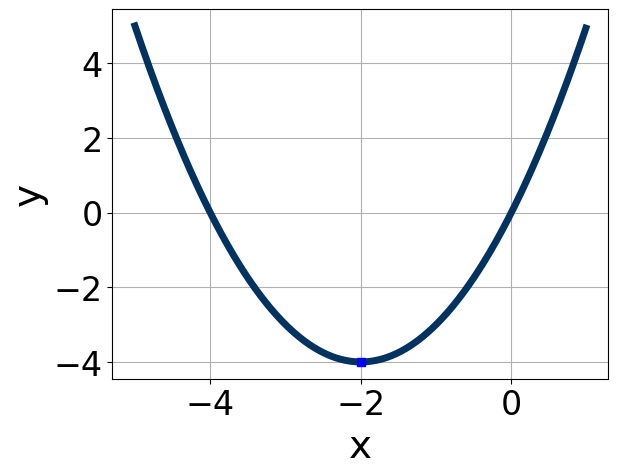
\includegraphics[width=0.5\textwidth]{../Figures/quadraticGraphToEquationCopyC.png}
\end{center}
\begin{enumerate}[label=\Alph*.]
\item \( a \in [1, 3], \hspace*{5mm} b \in [-8, -5], \text{ and } \hspace*{5mm} c \in [24, 25] \)
\item \( a \in [-1, 0], \hspace*{5mm} b \in [8, 11], \text{ and } \hspace*{5mm} c \in [-11, -5] \)
\item \( a \in [-1, 0], \hspace*{5mm} b \in [-8, -5], \text{ and } \hspace*{5mm} c \in [-11, -5] \)
\item \( a \in [1, 3], \hspace*{5mm} b \in [8, 11], \text{ and } \hspace*{5mm} c \in [24, 25] \)
\item \( a \in [1, 3], \hspace*{5mm} b \in [-8, -5], \text{ and } \hspace*{5mm} c \in [5, 11] \)

\end{enumerate} }
\litem{
Factor the quadratic below. Then, choose the intervals that contain the constants in the form $(ax+b)(cx+d); b \leq d.$\[ 54x^{2} +57 x + 10 \]\begin{enumerate}[label=\Alph*.]
\item \( a \in [1.9, 4.7], \hspace*{5mm} b \in [2, 5], \hspace*{5mm} c \in [16.9, 18.5], \text{ and } \hspace*{5mm} d \in [3, 8] \)
\item \( a \in [-0.1, 1.1], \hspace*{5mm} b \in [10, 14], \hspace*{5mm} c \in [-0.5, 1.5], \text{ and } \hspace*{5mm} d \in [45, 49] \)
\item \( a \in [7.6, 10.3], \hspace*{5mm} b \in [2, 5], \hspace*{5mm} c \in [4.3, 7], \text{ and } \hspace*{5mm} d \in [3, 8] \)
\item \( a \in [24.8, 27.9], \hspace*{5mm} b \in [2, 5], \hspace*{5mm} c \in [1.3, 5.3], \text{ and } \hspace*{5mm} d \in [3, 8] \)
\item \( \text{None of the above.} \)

\end{enumerate} }
\litem{
Write the equation of the graph presented below in the form $f(x)=ax^2+bx+c$, assuming  $a=1$ or $a=-1$. Then, choose the intervals that $a, b,$ and $c$ belong to.
\begin{center}
    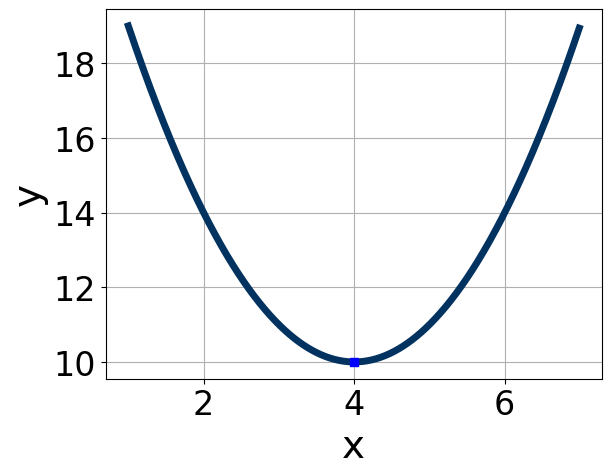
\includegraphics[width=0.5\textwidth]{../Figures/quadraticGraphToEquationC.png}
\end{center}
\begin{enumerate}[label=\Alph*.]
\item \( a \in [-0.2, 2.1], \hspace*{5mm} b \in [-12, -4], \text{ and } \hspace*{5mm} c \in [10, 11] \)
\item \( a \in [-1.4, -0.3], \hspace*{5mm} b \in [-12, -4], \text{ and } \hspace*{5mm} c \in [-11, -6] \)
\item \( a \in [-0.2, 2.1], \hspace*{5mm} b \in [8, 9], \text{ and } \hspace*{5mm} c \in [21, 23] \)
\item \( a \in [-1.4, -0.3], \hspace*{5mm} b \in [8, 9], \text{ and } \hspace*{5mm} c \in [-11, -6] \)
\item \( a \in [-0.2, 2.1], \hspace*{5mm} b \in [-12, -4], \text{ and } \hspace*{5mm} c \in [21, 23] \)

\end{enumerate} }
\litem{
Solve the quadratic equation below. Then, choose the intervals that the solutions $x_1$ and $x_2$ belong to, with $x_1 \leq x_2$.\[ 20x^{2} +21 x -54 = 0 \]\begin{enumerate}[label=\Alph*.]
\item \( x_1 \in [-2.21, -0.53] \text{ and } x_2 \in [3.58, 3.65] \)
\item \( x_1 \in [-10.1, -8.13] \text{ and } x_2 \in [0.16, 0.36] \)
\item \( x_1 \in [-45.55, -44.54] \text{ and } x_2 \in [23.98, 24.04] \)
\item \( x_1 \in [-2.7, -1.57] \text{ and } x_2 \in [1.1, 1.3] \)
\item \( x_1 \in [-8.22, -5.57] \text{ and } x_2 \in [0.32, 0.42] \)

\end{enumerate} }
\litem{
Factor the quadratic below. Then, choose the intervals that contain the constants in the form $(ax+b)(cx+d); b \leq d.$\[ 24x^{2} +38 x + 15 \]\begin{enumerate}[label=\Alph*.]
\item \( a \in [3.4, 6.3], \hspace*{5mm} b \in [-3, 6], \hspace*{5mm} c \in [4.7, 8.3], \text{ and } \hspace*{5mm} d \in [3, 7] \)
\item \( a \in [0.6, 3.5], \hspace*{5mm} b \in [16, 24], \hspace*{5mm} c \in [0.5, 1.8], \text{ and } \hspace*{5mm} d \in [13, 24] \)
\item \( a \in [7, 8.3], \hspace*{5mm} b \in [-3, 6], \hspace*{5mm} c \in [1.5, 4.4], \text{ and } \hspace*{5mm} d \in [3, 7] \)
\item \( a \in [0.6, 3.5], \hspace*{5mm} b \in [-3, 6], \hspace*{5mm} c \in [17.3, 18.6], \text{ and } \hspace*{5mm} d \in [3, 7] \)
\item \( \text{None of the above.} \)

\end{enumerate} }
\litem{
Solve the quadratic equation below. Then, choose the intervals that the solutions belong to, with $x_1 \leq x_2$ (if they exist).\[ 15x^{2} +9 x -2 = 0 \]\begin{enumerate}[label=\Alph*.]
\item \( x_1 \in [-11.71, -10.95] \text{ and } x_2 \in [2.21, 2.91] \)
\item \( x_1 \in [-1.03, -0.44] \text{ and } x_2 \in [-0.35, 0.73] \)
\item \( x_1 \in [-0.58, 0.38] \text{ and } x_2 \in [0.56, 0.92] \)
\item \( x_1 \in [-14.51, -14.09] \text{ and } x_2 \in [13.67, 14.35] \)
\item \( \text{There are no Real solutions.} \)

\end{enumerate} }
\litem{
Graph the equation below.\[ f(x) = -(x+1)^2 - 15 \]\begin{enumerate}[label=\Alph*.]
\begin{multicols}{2}\item 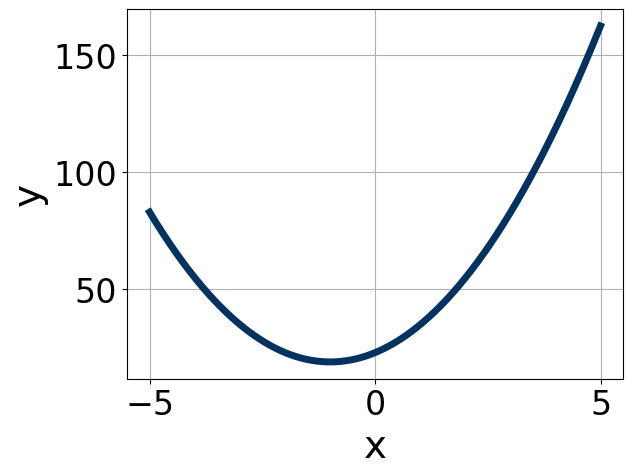
\includegraphics[width = 0.3\textwidth]{../Figures/quadraticEquationToGraphCopyAC.png}\item 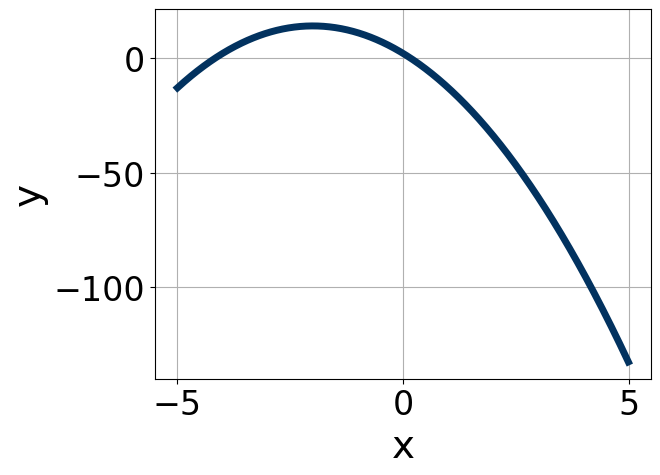
\includegraphics[width = 0.3\textwidth]{../Figures/quadraticEquationToGraphCopyBC.png}\item 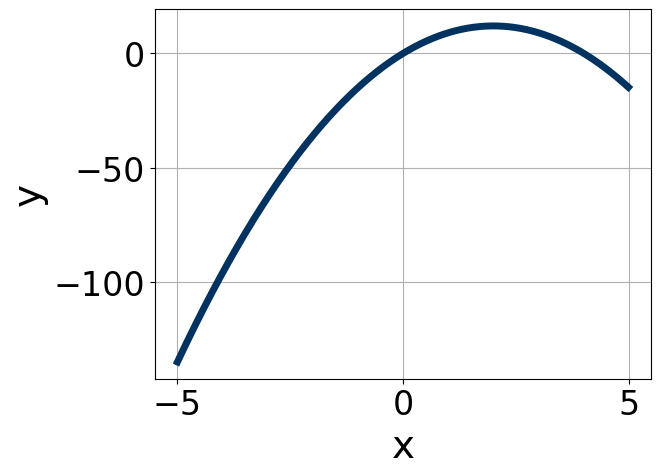
\includegraphics[width = 0.3\textwidth]{../Figures/quadraticEquationToGraphCopyCC.png}\item 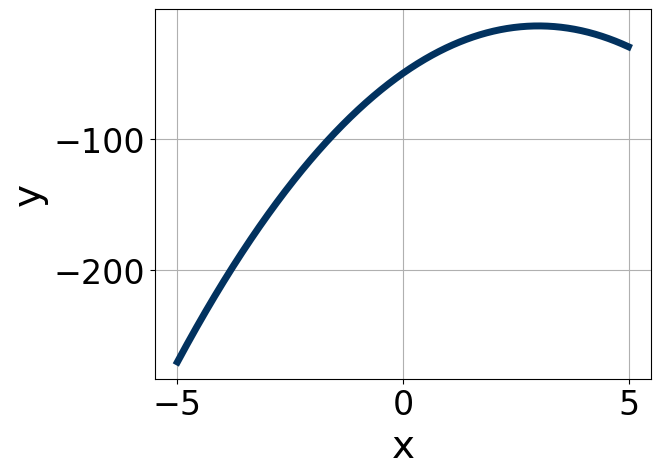
\includegraphics[width = 0.3\textwidth]{../Figures/quadraticEquationToGraphCopyDC.png}\end{multicols}\item None of the above.
\end{enumerate} }
\end{enumerate}

\end{document}